% :encoding=UTF-8:
% -*- TeX:UK -*-
\documentclass[12pt,oneside]{paper}
\usepackage{authblk}
\usepackage[datesep={},hourminsep={},useregional]{datetime2}
\usepackage{amsmath,bm}
\usepackage[
	xetex,
	bookmarks=true,bookmarksopen,
	colorlinks=true,citecolor=blue,urlcolor=BleuTor,linkcolor=black,
	pdfauthor={Vincent BAIN},
	pdftitle={r.avac manual},
	pdfsubject={computing flowing avalanches using AVAC: coupling with GRASS GIS}]{hyperref}
	

\hypersetup{
pdfinfo={
CreationDate={D:201910221700},
ModDate={D:\DTMnow}
}
}
\usepackage[
	a4paper,
	vscale=1,
	top=2.5cm,
	bottom=2.5cm,
	left=2.5cm,
	right=2.5cm]{geometry}
\usepackage[T1]{fontenc}
\usepackage{french}
\usepackage{color}
\usepackage[xetex]{graphicx}
\usepackage{fancyhdr}
\usepackage{titlesec}
\usepackage{fancyvrb}
\usepackage{manfnt}

\definecolor{gris.3}{gray}{0.3}
\definecolor{gris.5}{gray}{0.5}
\definecolor{noir}{gray}{0}
\definecolor{BleuTor}{rgb}{0,0.53,0.72}

\titleformat*{\subsection}{\bfseries}
\titleformat*{\paragraph}{\bfseries}

\newcommand{\esp}{\vskip0.3cm}
\newcommand{\comment}[1]{\marginpar{\begin{flushleft}  #1\end{flushleft}}}

\newenvironment{code}{%
\vspace{2mm}%
\hangindent=.6cm%
\parindent.6cm%
\ttfamily%
\color{gris.3}%
}{
\vspace{2mm}%
}

\makeatletter
\addto\captionsfrench{\renewcommand{\fnum@figure}{\small\textbf{\figurename~\thefigure}}}
\makeatother

\addto\captionsfrench{\def\figurename{{\small Figure}}}
\addto\captionsfrench{\def\CaptionSeparator{. \space}}
\def\captionseparator{. \space}
\addto\captionsfrench{\def\captionfont{\small}}

%fontes
%..............................
\usepackage{fontspec}
\defaultfontfeatures{Mapping=tex-text}
\setmainfont[
BoldFont = LinLibertine_RB.otf,
ItalicFont = LinLibertine_RI.otf,
BoldItalicFont = LinLibertine_RBI.otf
]{LinLibertine_R.otf}
\setsansfont[SmallCapsFont = Fontin SmallCaps,BoldFont = Fontin Bold]{Fontin}
%..............................


\newcommand{\bei}{\begin{itemize}}
\newcommand{\eit}{\end{itemize}}


\makeatletter
\let\ps@plain\ps@fancy
\makeatother

\fancyhead{}
\fancyfoot{}
\renewcommand*{\headrulewidth}{0pt}
\renewcommand*{\footrulewidth}{0pt}

\fancyhead[C]{\includegraphics[width=2.5cm]{toraval.eps}}
\fancyfoot[C]{\color{gris.5}\small{\textsf{\texttt{\large{r.avac}} (version 3.1.3) manual }\hfill\thepage}}


\begin{document}
\english 
\pagestyle{fancy}
\title{Computing flowing avalanches using AVAC: the r.avac  GRASS module}
\subtitle{October 2020}
\date{\today}
\author[1]{Vincent Bain}
\affil[1]{\small Toraval France, 2838 route des Annuits, F-73400 Ugine}
\date{October 2020}

\maketitle
\section{Introduction}

The AVAC code is used to run numerical simulations of flowing avalanches. It is based on the \href{https://www.clawpack.org/}{\textsc{ClawPack}} software and its \href{https://www.clawpack.org/geoclaw.html}{\textsc{GeoClaw}} library. Preparing the input data and displaying the output files may be difficult. Here we propose an additional module to the GRASS geographic information system (GRASS AddOn) called \verb+r.avac+. This document provides instructions for a quick start.

The \verb+r.avac+ module involves several programs commonly found in GNU/Linux repositories. It has not been tested for Mac OS and Windows operating systems. The easiest way to avoid compatibility problems is probably to work on a workstation running under GNU/Linux, physically or virtually (e.g., Oracle VM VirtualBox).



\section{Prerequisites}

We assume that the users have followed the installation instructions for the AVAC code, i.e. they have a functional Clawpack environment, in particular:
\bei
\item The environment variable \$CLAW points to the Clawpack installation directory.
\item the \texttt{qinit\_module.f90} file located in the \texttt{\$CLAW/geoclaw/src/2d/shallow} directory has been correctly modified (see AVAC documentation).
\eit

You must install the GNU/parallel and OpenMP programs in order to take advantage of parallelisation.

Finally, the \verb+r.avac+ module requires the Temporary features of GRASS GIS, so it is advisable to use a GRASS version higher than 7.0.

 

\section{Installation}
Clone the GitHub \href{https://github.com/xyleme/ravac}{ravac} repository

\begin{code}
git clone https://github.com/xyleme/avac

cd ravac
\end{code}

The \texttt{ravac} directory contains three elements:
\begin{itemize}
\item The directory named \texttt{avac}, which must be moved into the geoclaw \texttt{examples/} directory:

\begin{code}
mv avac/ \$AVAC/geoclaw/examples/
\end{code}

\item The \texttt{r.avac} executable file, which must be moved into a directory recognized by GRASS GIS (and thus be included as an AddOn source). The module in its current version does not appear in the official GRASS GIS repositories, so it cannot be installed from the \texttt{g.extension} utility.
Rather than placing \texttt{r.avac} in the dedicated directory (\texttt{\textasciitilde/.grass7/addons/bin/}) we prefer to place it in a separate directory \texttt{/usr/local/grass-addons/}:
\begin{code}
\$ mkdir /usr/local/grass-addons/

\$ mv r.avac /usr/local/grass-addons/
\end{code}
then declare the corresponding environment variable in the \texttt{.bashrc} file  (if the system shell is bash), as follows:
\begin{code}
export GRASS\_ADDON\_PATH=/usr/local/grass-addons/
\end{code}

\item The \texttt{boussolenc.gpkg} file which contains a set of cartographic data that can be used to test \verb+r.avac+ .
\end{itemize}

 

\section{Input data preparation}

As stated in the preamble,  the \verb+r.avac+ module aims to simplify the use of AVAC by providing the user with simple tools for preparing the required input data and defining model parameters. GRASS provides an appropriate framework and routines to that end. The user familiar with GIS---and in particular GRASS---can refer directly to the following section, in which we detail the procedure to run the code.

\subsection{Location and Mapset}

GRASS requires a set of files that defines the reference map coordinate system (directory named \emph{Location}) and data sets (subdirectories \emph{Mapsets}). Let us consider that we are working on a slope located in the French Alps, therefore we use the Lambert 93 coordinate system, and create an L93 location. When the program is started in graphical mode for the first time, a sequence of steps guides the user in determining a suitable reference system (see figure \ref{fig:location}). The program suggests creating a mapset, which has the user's name by default.


\begin{figure}[!h]
\begin{center}
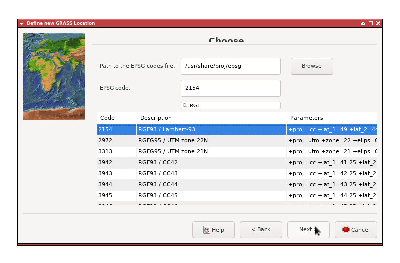
\includegraphics[width=0.70\hsize]{capture0.eps}
\caption{The procedure for creating a location in GRASS GIS asks the user to specify a reference coordinate system.}
\label{fig:location}
\end{center}
\end{figure}

This step can also be executed from the command window using the following command:

\begin{code}
grass79 -c EPSG:2154 L93
\end{code}

GRASS GIS allows the user to manage raster data, vector data and attribute data. The \verb+r.avac+ module uses these three types of data.

\subsection{Raster data: importation of topographical data}
The \texttt{boussolenc.gpkg} file is a geopackage whose data are georeferenced in the Lambert 93 system. It includes a \emph{digital elevation model} (DEM) named \texttt{topo}, and a shaded relief map named \texttt{shading} that we will import into our location by typing the following command lines in the command window:

\begin{code}
r.in.gdal input=boussolenc.gpkg gdal\_doo='table=topo\_2m' output=topo

r.in.gdal input=boussolenc.gpkg gdal\_doo='table=ombrage' output=shade
\end{code}

In the \emph{Layer Manager} window, the user can add these maps to the current view (see figure \ref{fig:shade}).

\begin{figure}[!h]
\begin{center}
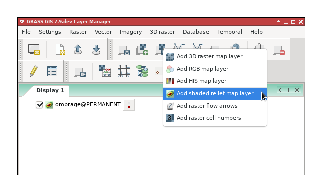
\includegraphics[width=0.70\hsize]{capture3.eps}
\caption{The \emph{Add various raster map layers > Add shaded relief map} menu makes it possible to combine shaded relief and DEM.}
\label{fig:shade}
\end{center}
\end{figure}

To provide AVAC with the desired topographic data, \verb+r.avac+ transforms the raster map and passes it on to the code by means of the file named \texttt{topo.asc}. The resolution and geographical extension of this file are controlled by the user when defining the working region.


\subsection{Notion of region}

A central notion of GRASS GIS is the \emph{region}. It is a set of numerical values indicating the position, range, and resolution of a grid that discretises the working area (or computational domain). By default in a blank location, this region is defined by a single cell located at the origin of the current projection's  Cartesian frame. \comment{\dbend}\textbf{If we want GRASS to process our data properly, it is essential to indicate the region parameters related to the working area}. In this case,  run the following command to make the region coincide with the extension and resolution of the digital elevation model (imported during the previous step):

\begin{code}
g.region -p rast=topo
\end{code}

The \texttt{-p} option forces to display the new region parameters in the output.

The map display window allows the user to view the current region (see figure \ref{fig:raster}). The user can also define the region extension interactively in the map display window (Various zoom options icon > set computational region extent interactively).

Finally, it is possible, and desirable, to determine the resolution on which we wish to work. The previous command tells us that the sampling step of the topography we imported is 2\,m. We can decide to work with a mesh grid of 5\,m, by giving the following instruction:

\begin{code}
g.region -pa res=5
\end{code}

The \texttt{-a} option forces the region definition by imposing that its dimensions are proportional to the desired resolution.

\begin{figure}[!h]
\begin{center}
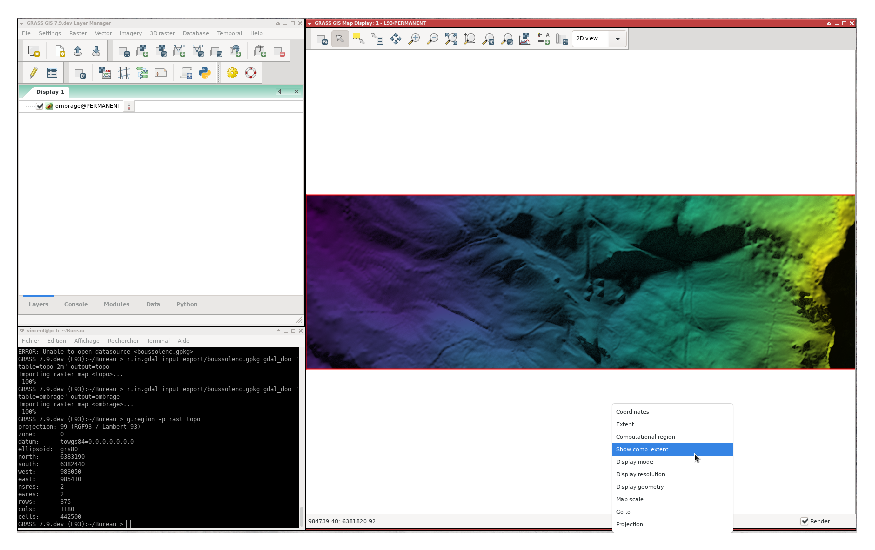
\includegraphics[width=1\hsize, angle=00]{capture1.eps}
\caption{Shaded relief display of the digital elevation model. The \emph{map display} window displays the current region as a red frame.}
\label{fig:raster}
\end{center}
\end{figure}

The current version of \verb+r.avac+ rpovides a rough support of AMR (adaptive mesh refinement) functionality; ordering GeoClaw to work locally at a given AMR can be done by specifying a rectangular area (via \verb+amr+ option) previously set within GRASS GIS: the user determines a rectangular polygon which category (\verb+cat+) stands for theamr wished level (the current version only support level 2). A quite handy way to proceed is as follows:
\bei
\item interactively define a new region in the map display (see above);
\item create a vector map sourced from this new region setup: 

\begin{code}
v.in.region cat=2 out=amr2 --o
\end{code}
\eit

\subsection{Vector data: creation of a vector map}

The file named \texttt{boussolenc.gpkg} is a geographic dataset containing among others a contour level layer, which is easily imported in GRASS GIS:

\begin{code}
v.in.ogr in=boussolenc.gpkg layer='cbn' out=cbn
\end{code}

On top of the previously imported raster stack, it provides a neat perception of terrain shape.

The AVAC code needs to know the location of the avalanche starting area(s), as well as the initial height of snow mobilised in each area. The \texttt{r.avac} module provides these initial data in the form of a vector map called \texttt{ZA}, comprising as many polygons as there are starting zones. The initial snow height in each area is contained in the attribute called \texttt{h}.

The \texttt{boussolenc.gpkg} file includes an example of a vector layer named \texttt{ZA} in the format expected by \verb+r.avac+. To import it into GRASS, run the following command line:


\begin{code}
v.in.ogr in=boussolenc.gpkg layer='ZA' out=ZA
\end{code}

The following commands ensure that the \texttt{h} field is present in the ZA layer's attribute table:

\begin{code}
v.db.connect ZA -p

db.columns ZA
\end{code}

The user is referred to the GRASS GIS documentation for further information, in particular for a presentation of:
 \begin{itemize}
 \item  vector models \href{https://grass.osgeo.org/grass76/manuals/vectorintro.html}{https://grass.osgeo.org/grass76/manuals/vectorintro.html}, 
  \item attributes \href{https://grasswiki.osgeo.org/wiki/Vector\_Database\_Management}{https://grasswiki.osgeo.org/wiki/Vector\_Database\_Management}, and
  \item the editing tools \footnote{\href{https://grass.osgeo.org/grass76/manuals/wxGUI.vdigit.html}{https://grass.osgeo.org/grass76/manuals/wxGUI.vdigit.html}}  (see figure \ref{fig:vector}).
\end{itemize}

\begin{figure}[!h]
\begin{center}
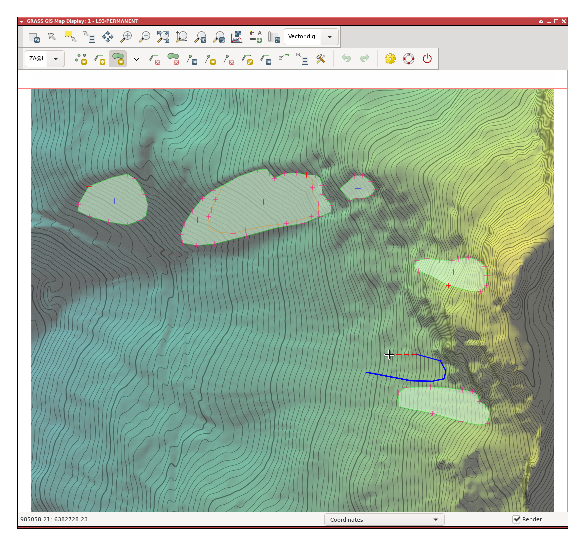
\includegraphics[width=0.70\hsize]{capture2.eps}
\caption{The ZA vector layer can be edited to modify, add, delete start areas.}
\label{fig:vector}
\end{center}
\end{figure}

To provide AVAC with the required input data,  \verb+r.avac+ discretises the vector map and passes it on to the code via the file named \texttt{initials.xyz}.

\subsection{r.avac features}

\paragraph{Rheologic law}
AVAC code allows to choose between two snow rheologies. Friction can be expressed:
\bei
\item either by a \emph{Voellmy} law (with two parameters $\mu$, $\xi$), or
\item by a \emph{Coulomb} law (with a single parameter$\mu$).
\eit

The user tells \verb+r.avac+ which law to use providing the \verb+rheology+ argument:
\bei
\item \texttt{rheology=0} stands for Voellmy, the default value ;
\item \texttt{rheology=1} stands for Coulomb.
\eit
Choosing \verb+rheology=1+ cancels $\xi$ parameter.

\paragraph{Snow heights}
In this version \verb+r.avac+ can modulate the snow height, provided by the \verb+depth+ parameter or the \verb+h+ vector attribute, taking into account the local steepness of the slope in the starting area. The program uses a modified version of the de Qervain formula:
\[
h(z) = h_0(z) \frac{\sin\theta_{ref}-\nu \cos\theta_{ref}}{\sin\theta -\nu \cos\theta},
\]

where $h_0$ is the snow depth (on a flat ground) at a $z$ given altitude, $\theta_{ref}$ is a reference angle (slope for which the correction factor is 1), $\theta$ is the slope angle of the starting area at the $z$ altitude, and $snu$ is an empirical coefficient. Default values $\nu=0,2$ and $\theta_{ref}=30$ can be tweaked inside the \verb+r.avac+ source code.

In addition, this version of \verb+r.avac+ allows to fine tune snow depths in the starting area by specifying a hypsometric gradient thanks the \verb+grad+ argument, expressed as a triplet (depth,gradient,altitude), e.g.


\begin{code}
\texttt{grad=1.8,0.03,1850} 
\end{code}

means the snow depth is 180\,cm at 1850\,m, and the hypsometric gradient is 3\,cm per 100\,m elevation. Giving this option to \verb+r.avac+ the initial condition grid values override any value provided by \verb+depth+ parameter or the \verb+h+ vector attribute.

\section{Running r.avac}

\subsection{Syntax}

\verb+r.avac+ can be executed at the terminal . For a first use, it may be more convenient to use the module's user interface. To that end, simply run at the grass prompt:
\begin{code}
r.avac --ui
\end{code}

Every argument in the \emph{Required} tab must be filled. The \emph{Optional} tab contains arguments whose values are set by default, including the AVAC model calibration parameters (see AVAC documentation).


%\clearpage
The \texttt{--h} option yields the command's full syntax:

\begin{code}
r.avac --h
\begin{Verbatim}
Usage:
 r.avac [-mrc] simul=name dem=name za=name [depth=name] [amr=name]
   [dt=string] [t=string] [rheology=string] [rho=string] [xi=string]
   [mu=string] [grad=string] [vthres=string] [bslope=string]
   [--overwrite] [--help] [--verbose] [--quiet] [--ui]

Flags:
  -m   compute max(h) and max(p) maps throughout simul strds
  -r   reset existing simul strds
  -c   run geoclaw 'make clobber'
  -a   run r.avac in amnesiac mode (make sure -m flag is on)

Parameters:
     simul   output simulation STRDS
       dem   input elevation raster map
        za   input starting area vector map
     depth   depth column for starting area
       amr   input AMR zone map
        dt   time increment
             default: 20
         t   simulation duration
             default: 100
  rheology   type of rheology
             default: 0
       rho   snow density
             default: 300
        xi   Voellmy xi
             default: 1500
        mu   Voellmy mu
             default: 0.15
      grad   depth hypsometric gradient
    vthres   velocity threshold
             default: 0.05
    bslope   beta slope
             default: 1.1
\end{Verbatim}
\end{code}

With a little practice, the user may prefer to execute \verb+r.avac+ from the GRASS console. For example:

\french
\begin{code}
r.avac -mr simul=sim2 rheology=0 dem=topo za=ZA dt=1 t=40 \backslash

mu=0.2 xi=800 rho=300 grad=1.7,0.03,1850 amr=amr2 vthres=0.2
\end{code}
\english

The advantage of using the command line rather than the user interface is that it is easier to do several iterations of the code by changing one or several parameters. Taking advantage of the command line history in the GRASS command window makes things easier.

\subsection{How it works}

When the command is run, the script provides the AVAC code with topographic data (\verb+topo.asc+), initial conditions (\verb+initial.xyz+), computational domain (according to the region parameters previously defined), and the computation parameters in \verb+voellmy.data+, \verb+AddSetrun.py+, and \verb+setrun.py+ files.

Once the computation has been done, \verb+r.avac+ processes the files \texttt{fort.qxxxx} produced by AVAC in order to import the flow depth $h(t)$ and kinetic pressure $p(t)=\frac{1}{2}\varrho u^2$ into GRASS, where $\varrho$ and $u$ are the snow density and velocity, respectively. The tiles generated by the code are then stitched to obtain a set of rasters describing the flow at the time step \texttt{dt} prescribed in the input file. Using the previous command example, rasters named \texttt{h.sim2\_xxxx} and \texttt{p.sim2\_xxxx} are incorporated respectively in rasters time series (spatial temporal raster dataset, strds): one named \texttt{sim2\_h} describing the flow depth (expressed in m), the other named \texttt{sim2\_p} describing the kinetic pressure $p$ (expressed in kPa).

If the user wishes to interrupt the execution of the code, he can do so in graphic mode by pressing the Stop button. In line command,  the $<$ctrl+c$>$ shortcut stops the computations. The script performs cleaning operations before leaving (purging some parameters, deleting temporary files).

\section{Visualisation and export}

The user can visualise the simulation output by launching the interactive \texttt{g.gui.animation} module.

The colorimetric chart associated with each series can easily be modified. For example, if the user want to apply the pressure chart used in Toraval documents, which is recorded in the \texttt{p\_toraval.file} file attached to our archive:

\begin{code}
t.rast.colors input=sim5\_h rules=[/path\_to/]p\_toraval.file
\end{code}


The \texttt{g.gui.animation} module offers the possibility to export animations in several forms. When the number of maps in the time series is large (typically a thousand files), it is no longer possible to view or export the series. The user can then choose to export a series of images in png format for post-processing with other tools, such as the \verb+ffmpeg+ software:

\french
\begin{code}
\begin{Verbatim}
g.list rast | grep h.sim2 | parallel r.out.png in={} out={}
ffmpeg -f image2 -r 12 -i "h.sim2_0\%03d.png" -vcodec png out_h.avi

g.list rast | grep p.sim2 | parallel r.out.png in={} out={}
ffmpeg -f image2 -r 12 -i "p.sim2_0\%03d.png" -vcodec png out_p.avi
\end{Verbatim}
\end{code}
\english


\newpage

~\vfill

\begin{figure}[!h]
\begin{center}
\includegraphics[width=0.70\hsize]{capture4.eps}
\caption{Example of post-processing performed using \href{https://www.blender.org/}{Blender} to produce an animation combining flow depth (displacement) and pressure (color). See video at \href{http://telec.toraval.fr/boussolenc.avi}{http://telec.toraval.fr/boussolenc.avi}}.
\label{fig:blend}
\end{center}
\end{figure}

~\vfill

\end{document}
